%==============================================================
%  Retrieval-Augmented Generation (RAG) -- explained from zero
%  A Beamer presentation for a non-technical audience.
%
%  Animated version: diagrams and lists build up step by step,
%  slide 15 plays a real auto-running animation.
%
%  Compile with:  pdflatex rag-presentation.tex   (run twice)
%  Present in your PDF viewer's fullscreen / presentation mode.
%==============================================================
\documentclass[aspectratio=169,11pt]{beamer}

\usetheme{Madrid}
\usecolortheme{whale}
\setbeamertemplate{navigation symbols}{}

\usepackage[T1]{fontenc}
\usepackage[utf8]{inputenc}
\usepackage{lmodern}
\usepackage{tikz}
\usepackage{amssymb}
\usetikzlibrary{arrows.meta,positioning,shapes.geometric,calc,fit,backgrounds}

%---------------- colour palette -------------------------------
\definecolor{ragblue}{RGB}{31,84,142}
\definecolor{raglight}{RGB}{225,236,247}
\definecolor{ragorange}{RGB}{214,124,29}
\definecolor{ragsand}{RGB}{252,240,222}
\definecolor{raggreen}{RGB}{40,124,86}
\definecolor{ragmint}{RGB}{224,240,232}
\definecolor{ragred}{RGB}{176,58,58}
\definecolor{raggray}{RGB}{100,100,100}

\setbeamercolor{structure}{fg=ragblue}
\setbeamercolor{palette primary}{bg=ragblue,fg=white}
\setbeamercolor{title}{bg=ragblue,fg=white}
\setbeamercolor{frametitle}{bg=ragblue,fg=white}
\setbeamercolor{block title}{bg=ragblue,fg=white}
\setbeamercolor{block body}{bg=raglight,fg=black}
\setbeamercolor{block title alerted}{bg=ragred,fg=white}
\setbeamercolor{block title example}{bg=raggreen,fg=white}
\setbeamercolor{block body example}{bg=ragmint,fg=black}
\setbeamerfont{frametitle}{series=\bfseries}
\setbeamerfont{title}{series=\bfseries}
\setbeamertemplate{itemize item}{\color{ragblue}$\blacktriangleright$}
\setbeamertemplate{itemize subitem}{\color{ragorange}$\bullet$}
\setbeamertemplate{caption}[numbered]

% compact footline: author | title | frame number
\setbeamertemplate{footline}{%
  \hbox{%
  \begin{beamercolorbox}[wd=.32\paperwidth,ht=2.4ex,dp=1.2ex,left,leftskip=1em]{author in head/foot}%
    \usebeamerfont{author in head/foot}\insertshortauthor
  \end{beamercolorbox}%
  \begin{beamercolorbox}[wd=.53\paperwidth,ht=2.4ex,dp=1.2ex,center]{title in head/foot}%
    \usebeamerfont{title in head/foot}\insertshorttitle
  \end{beamercolorbox}%
  \begin{beamercolorbox}[wd=.15\paperwidth,ht=2.4ex,dp=1.2ex,right,rightskip=1em]{date in head/foot}%
    \usebeamerfont{date in head/foot}\insertframenumber\,/\,\inserttotalframenumber
  \end{beamercolorbox}}%
}

%---------------- reusable tikz styles -------------------------
\tikzset{
  box/.style   = {rounded corners=3pt, draw=ragblue, thick, fill=raglight,
                  align=center, inner sep=6pt, minimum height=1cm, font=\small},
  obox/.style  = {box, draw=ragorange, fill=ragsand},
  gbox/.style  = {box, draw=raggreen, fill=ragmint},
  rbox/.style  = {box, draw=ragred, fill=red!8},
  doc/.style   = {draw=raggray, fill=white, minimum width=1.1cm,
                  minimum height=1.4cm, font=\tiny, align=center},
  ar/.style    = {-{Stealth[length=2.4mm]}, thick, draw=raggray},
  lbl/.style   = {font=\scriptsize\itshape, text=raggray},
}

% ---- overlay-aware TikZ ---------------------------------------
% "visible on=<2->" hides a node/path on other slides WITHOUT
% removing it, so nothing shifts as the diagram builds up.
\tikzset{
  invisible/.style   = {opacity=0},
  visible on/.style  = {alt={#1{}{invisible}}},
  alt/.code args     = {<#1>#2#3}{%
    \alt<#1>{\pgfkeysalso{#2}}{\pgfkeysalso{#3}}%
  },
}

% length register driven by \animatevalue on the animated slide
\newlength{\searchradius}

% one point on the map of meaning: it lights up once the growing
% search radius has passed its distance from the query.
% #1 x  #2 y  #3 label  #4 distance from query  #5 label placement
\newcommand{\swallowpoint}[5]{%
  \ifdim\searchradius>#4\relax
    \fill[ragblue] (#1,#2) circle (3.2pt);
    \node[font=\scriptsize\bfseries, text=ragblue, #5] at (#1,#2) {#3};
  \else
    \fill[raggreen] (#1,#2) circle (2.1pt);
    \node[font=\scriptsize, #5] at (#1,#2) {#3};
  \fi
}

%---------------- title data -----------------------------------
\title[RAG: Teaching AI to Look Things Up]{Retrieval-Augmented Generation (RAG)}
\subtitle{How we teach an AI to look things up before it answers}
\author[RAG Talk]{Adham}
\institute{}
\date{\today}

%---------------- section divider ------------------------------
\AtBeginSection[]{%
  \begin{frame}[plain]
    \transfade
    \vfill
    \centering
    \begin{beamercolorbox}[sep=10pt,center,rounded=true,shadow=true]{title}
      \usebeamerfont{title}\insertsectionhead
    \end{beamercolorbox}
    \vfill
  \end{frame}
}

\begin{document}

\begin{frame}[plain]
  \titlepage
  \begin{center}
    \small\color{raggray}
    No prior knowledge of AI assumed --- we start from zero.
  \end{center}
\end{frame}

%==============================================================
\begin{frame}{Where we are going}
  \tableofcontents[pausesections]
\end{frame}

\begin{frame}{The one-sentence version}
  \vfill
  \begin{block}{If you remember only one thing}
    \large
    RAG means: \textbf{before} the AI answers your question, we quickly
    \textbf{search} a trusted collection of documents, hand the AI the most
    relevant pages, and ask it to answer \textbf{using those pages}.
  \end{block}
  \vfill
  \begin{center}
  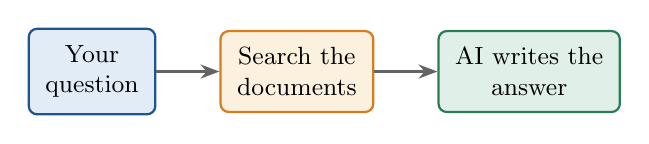
\begin{tikzpicture}[node distance=8mm]
    \node[box, visible on=<2->] (q) {Your\\question};
    \node[obox, right=of q, visible on=<3->] (s) {Search the\\documents};
    \node[gbox, right=of s, visible on=<4->] (a) {AI writes the\\answer};
    \draw[ar, visible on=<3->] (q) -- (s);
    \draw[ar, visible on=<4->] (s) -- (a);
  \end{tikzpicture}
  \end{center}
  \vfill
  \centering\small\color{raggray}
  \uncover<5->{Everything else in this talk explains \emph{how} and \emph{why}.}
\end{frame}

%==============================================================
\section{Part 1 --- What is an AI language model?}

\begin{frame}{Meet the language model}
  \begin{columns}[T,onlytextwidth]
    \begin{column}{0.525\textwidth}
      A \alert{Large Language Model} (LLM) --- the thing behind ChatGPT,
      Claude, Gemini --- does exactly one job:
      \begin{block}<2->{Its only skill}
        Given some text, predict what text should come next --- one word at a
        time, plausibly and fluently.
      \end{block}
      \medskip
      \uncover<4->{%
        It learned this by reading an enormous amount of text and noticing
        patterns:}
      \begin{itemize}
        \item<4-> how sentences are built,
        \item<4-> how ideas usually connect,
        \item<4-> a great deal of general world knowledge, absorbed along the way.
      \end{itemize}
    \end{column}
    \begin{column}{0.43\textwidth}
      \centering
      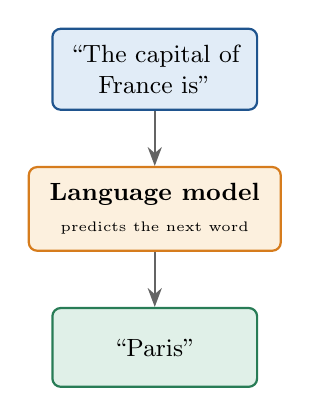
\begin{tikzpicture}[node distance=7mm]
        \node[box, minimum width=2.6cm, visible on=<2->] (in)
              {``The capital of\\France is''};
        \node[obox, below=of in, minimum width=3.2cm, visible on=<3->] (llm)
              {\textbf{Language model}\\\tiny predicts the next word};
        \node[gbox, below=of llm, minimum width=2.6cm, visible on=<3->] (out)
              {``Paris''};
        \draw[ar, visible on=<3->] (in) -- (llm);
        \draw[ar, visible on=<3->] (llm) -- (out);
      \end{tikzpicture}
      \medskip

      \small\color{raggray}
      \uncover<3->{Repeat this a few hundred times and you get a paragraph.}
    \end{column}
  \end{columns}
\end{frame}

\begin{frame}{A useful mental picture}
  \begin{block}{The brilliant intern who has read the whole library}
    Imagine hiring someone who has read millions of books and articles,
    writes beautifully, and answers instantly \dots
  \end{block}
  \medskip
  \begin{columns}[T,onlytextwidth]
    \begin{column}{0.478\textwidth}
      \begin{exampleblock}<2->{What they are great at}
        \begin{itemize}
          \item Explaining and summarising
          \item Writing, rewriting, translating
          \item General knowledge and reasoning
        \end{itemize}
      \end{exampleblock}
    \end{column}
    \begin{column}{0.478\textwidth}
      \begin{alertblock}<3->{\dots but}
        \begin{itemize}
          \item They read everything \emph{a while ago}
          \item They have \emph{never seen} your company's files
          \item They answer from \emph{memory}, and memory blurs
          \item They never say ``I am not sure''
        \end{itemize}
      \end{alertblock}
    \end{column}
  \end{columns}
\end{frame}

\begin{frame}{Problem 1 --- Frozen in time}
  A model's knowledge stops on the day its training data was collected.
  \bigskip
  \begin{center}
  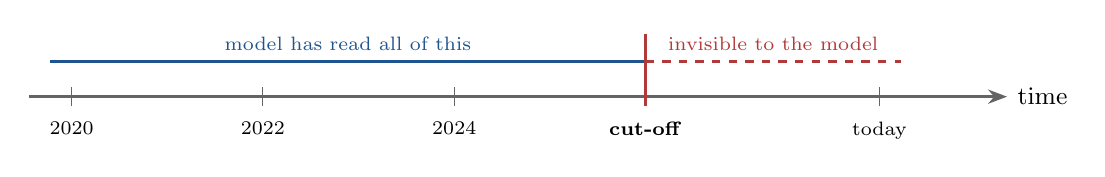
\begin{tikzpicture}[x=1.35cm]
    \draw[ar, line width=1pt] (0,0) -- (9.2,0) node[right,font=\small] {time};
    \foreach \x/\lbl in {0.4/2020, 2.2/2022, 4.0/2024, 5.8/{\textbf{cut-off}}, 8.0/today}{
      \draw[raggray] (\x,-0.12) -- (\x,0.12);
      \node[font=\scriptsize, below=1mm] at (\x,-0.1) {\lbl};
    }
    \draw[very thick, ragblue, visible on=<2->] (0.2,0.45) -- (5.8,0.45)
      node[midway, above, font=\scriptsize, text=ragblue] {model has read all of this};
    \draw[very thick, ragred, dashed, visible on=<3->] (5.8,0.45) -- (8.2,0.45)
      node[midway, above, font=\scriptsize, text=ragred] {invisible to the model};
    \draw[ragred, thick, visible on=<3->] (5.8,-0.12) -- (5.8,0.8);
  \end{tikzpicture}
  \end{center}
  \bigskip
  \begin{alertblock}<4->{Consequence}
    Yesterday's price change, this morning's policy update, last week's
    meeting notes --- the model simply does not know they exist.
  \end{alertblock}
\end{frame}

\begin{frame}{Problem 2 --- It has never seen \emph{your} documents}
  \begin{columns}[T,onlytextwidth]
    \begin{column}{0.497\textwidth}
      The model was trained on public text. It was never given:
      \begin{itemize}
        \item your internal policies and handbooks,
        \item your contracts and invoices,
        \item your product manuals,
        \item your patient, student or customer records.
      \end{itemize}
      \medskip
      \uncover<4->{And these are exactly the things people actually want to
      ask about.}
    \end{column}
    \begin{column}{0.458\textwidth}
      \centering
      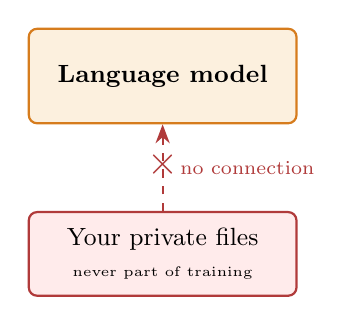
\begin{tikzpicture}
        \node[obox, minimum width=3.4cm, minimum height=1.2cm,
              visible on=<2->] (llm) {\textbf{Language model}};
        \node[rbox, below=1.1cm of llm, minimum width=3.4cm,
              visible on=<2->] (files)
             {Your private files\\\tiny never part of training};
        \draw[ar, ragred, dashed, visible on=<3->] (files) -- (llm)
          node[midway, right, font=\scriptsize, text=ragred] {\ no connection};
        \node[font=\Large, text=ragred, visible on=<3->]
              at ($(files)!0.5!(llm)$) {$\times$};
      \end{tikzpicture}
    \end{column}
  \end{columns}
\end{frame}

\begin{frame}{Problem 3 --- Confident invention (``hallucination'')}
  \begin{block}{Why it happens}
    The model is built to produce \emph{plausible} text, not \emph{verified}
    text. When it does not know, the machinery still runs --- and something
    plausible comes out.
  \end{block}
  \medskip
  \begin{columns}[T,onlytextwidth]
    \begin{column}{0.478\textwidth}
      \begin{alertblock}<2->{Typical symptoms}
        \begin{itemize}
          \item Invented rules, dates or numbers
          \item References to documents that do not exist
          \item A confident tone, either way
        \end{itemize}
      \end{alertblock}
    \end{column}
    \begin{column}{0.478\textwidth}
      \begin{exampleblock}<3->{The human analogy}
        A student in a closed-book exam who half-remembers the chapter and
        writes something that \emph{sounds} right rather than leaving
        the page blank.
      \end{exampleblock}
    \end{column}
  \end{columns}
  \medskip
  \centering
  \uncover<4->{\textbf{\color{ragblue}So: how do we let the student bring the
  book?}}
\end{frame}

%==============================================================
\section{Part 2 --- The RAG idea}

\begin{frame}{Closed book vs.\ open book}
  \begin{center}
  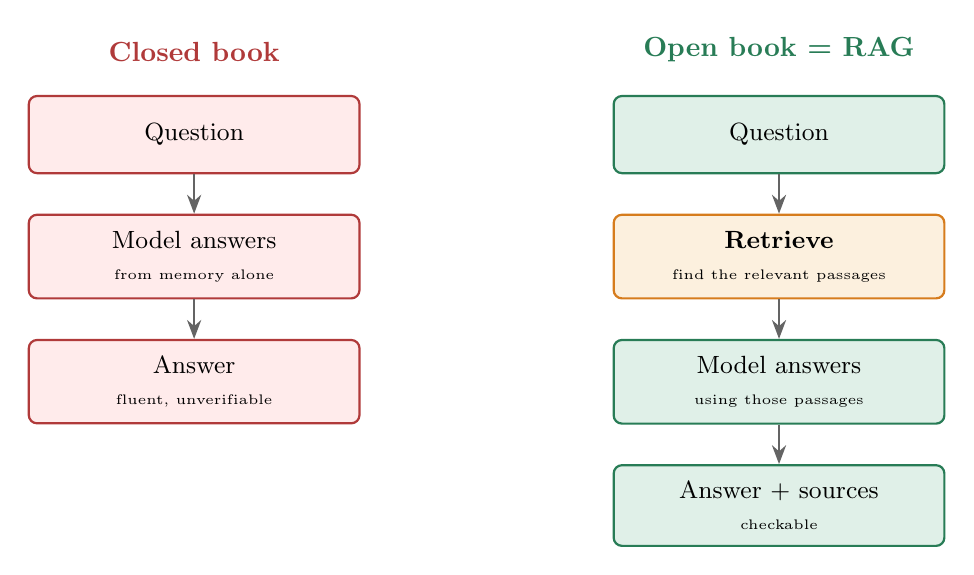
\begin{tikzpicture}[node distance=5mm]
    % closed book
    \node[rbox, minimum width=4.2cm, minimum height=0.98cm] (q1) {Question};
    \node[rbox, below=of q1, minimum width=4.2cm, minimum height=0.98cm] (m1)
         {Model answers\\\tiny from memory alone};
    \node[rbox, below=of m1, minimum width=4.2cm, minimum height=0.98cm] (a1)
         {Answer\\\tiny fluent, unverifiable};
    \draw[ar] (q1) -- (m1); \draw[ar] (m1) -- (a1);
    \node[above=3mm of q1, font=\bfseries, text=ragred] {Closed book};

    % open book -- built one step at a time
    \node[gbox, minimum width=4.2cm, minimum height=0.98cm, right=3.2cm of q1,
          visible on=<2->] (q2) {Question};
    \node[obox, below=of q2, minimum width=4.2cm, minimum height=0.98cm,
          visible on=<3->] (r2)
         {\textbf{Retrieve}\\\tiny find the relevant passages};
    \node[gbox, below=of r2, minimum width=4.2cm, minimum height=0.98cm,
          visible on=<4->] (m2)
         {Model answers\\\tiny using those passages};
    \node[gbox, below=of m2, minimum width=4.2cm, minimum height=0.98cm,
          visible on=<5->] (a2)
         {Answer $+$ sources\\\tiny checkable};
    \draw[ar, visible on=<3->] (q2) -- (r2);
    \draw[ar, visible on=<4->] (r2) -- (m2);
    \draw[ar, visible on=<5->] (m2) -- (a2);
    \node[above=3mm of q2, font=\bfseries, text=raggreen, visible on=<2->]
         {Open book = RAG};
  \end{tikzpicture}
  \end{center}
\end{frame}

\begin{frame}{Unpacking the name}
  \begin{center}
  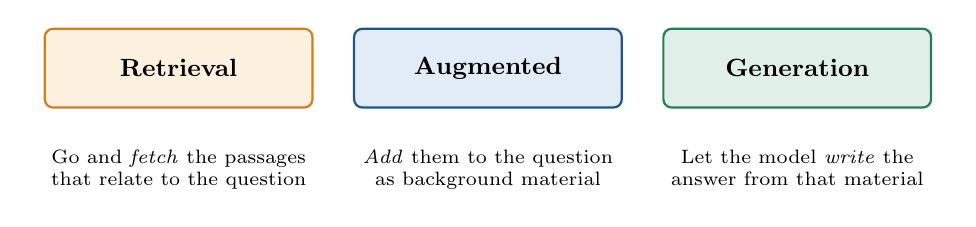
\begin{tikzpicture}[node distance=5mm]
    \node[obox, minimum width=3.4cm, visible on=<1->] (r) {\textbf{Retrieval}};
    \node[box,  minimum width=3.4cm, right=of r, visible on=<2->] (a)
         {\textbf{Augmented}};
    \node[gbox, minimum width=3.4cm, right=of a, visible on=<3->] (g)
         {\textbf{Generation}};
    \node[below=4mm of r, text width=3.6cm, align=center, font=\scriptsize,
          visible on=<1->]
      {Go and \emph{fetch} the passages that relate to the question};
    \node[below=4mm of a, text width=3.6cm, align=center, font=\scriptsize,
          visible on=<2->]
      {\emph{Add} them to the question as background material};
    \node[below=4mm of g, text width=3.6cm, align=center, font=\scriptsize,
          visible on=<3->]
      {Let the model \emph{write} the answer from that material};
  \end{tikzpicture}
  \end{center}
  \vfill
  \begin{exampleblock}<4->{The instruction we effectively give the model}
    ``Here are five passages from our handbook. Answer the user's question
    using \textbf{only} these passages, and tell me which one you used.
    If they do not contain the answer, say so.''
  \end{exampleblock}
\end{frame}

\begin{frame}{Why this fixes all three problems}
  \begin{columns}[T,onlytextwidth]
    \begin{column}{0.478\textwidth}
      \begin{alertblock}{Without RAG}
        \begin{itemize}
          \item Knowledge frozen at training time
          \item Blind to your private files
          \item Invents plausible details
          \item No way to check the answer
        \end{itemize}
      \end{alertblock}
    \end{column}
    \begin{column}{0.478\textwidth}
      \begin{exampleblock}<2->{With RAG}
        \begin{itemize}
          \item Reads today's documents at question time
          \item Your files \emph{are} the knowledge base
          \item Answers are anchored in real text
          \item Every answer can cite its source
        \end{itemize}
      \end{exampleblock}
    \end{column}
  \end{columns}
  \bigskip
  \begin{block}<3->{The key insight}
    We do not change the model at all. We change \textbf{what we put in front
    of it}. The model stays a general-purpose reader and writer; the
    documents supply the facts.
  \end{block}
\end{frame}

%==============================================================
\section{Part 3 --- How does a computer find ``relevant'' text?}

\begin{frame}{First attempt: search for the same words}
  Classic search matches the \emph{letters} you typed.
  \bigskip
  \begin{columns}[T,onlytextwidth]
    \begin{column}{0.478\textwidth}
      \begin{exampleblock}{Works fine}
        Question: ``\,\textbf{annual leave} policy''\\
        Document: ``Our \textbf{annual leave} policy states \dots''
      \end{exampleblock}
    \end{column}
    \begin{column}{0.478\textwidth}
      \begin{alertblock}<2->{Fails badly}
        Question: ``How many \textbf{days off} do I get?''\\
        Document: ``Employees accrue 21 days of \textbf{annual leave}.''\\
        \smallskip
        \emph{Zero words in common --- yet it is the right answer.}
      \end{alertblock}
    \end{column}
  \end{columns}
  \bigskip
  \begin{block}<3->{What we actually need}
    A way to match on \textbf{meaning}, not spelling --- so that
    \emph{days off}, \emph{vacation}, \emph{annual leave} and \emph{holiday
    allowance} all land in the same place.
  \end{block}
\end{frame}

\begin{frame}{The trick: turn meaning into coordinates}
  \begin{block}{Embedding}
    An \alert{embedding} is a list of numbers that represents the meaning of a
    piece of text. Similar meanings get similar numbers.
  \end{block}
  \medskip
  \begin{center}
  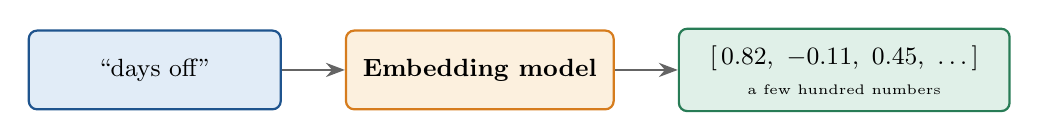
\begin{tikzpicture}[node distance=8mm]
    \node[box, minimum width=3.2cm, visible on=<2->] (t) {``days off''};
    \node[obox, right=of t, minimum width=3.4cm, visible on=<3->] (e)
         {\textbf{Embedding model}};
    \node[gbox, right=of e, minimum width=4.2cm, visible on=<4->] (v)
         {$[\,0.82,\ -0.11,\ 0.45,\ \dots\,]$\\\tiny a few hundred numbers};
    \draw[ar, visible on=<3->] (t) -- (e);
    \draw[ar, visible on=<4->] (e) -- (v);
  \end{tikzpicture}
  \end{center}
  \medskip
  \begin{columns}[T,onlytextwidth]
    \begin{column}{0.592\textwidth}
      \uncover<5->{Think of each list of numbers as an \textbf{address on a map
      of meaning}. Texts about the same topic end up in the same
      neighbourhood --- even with no shared words.}
    \end{column}
    \begin{column}{0.363\textwidth}
      \small\color{raggray}
      \uncover<5->{Nobody chooses these numbers by hand. The embedding model
      learned them from data, the same way the language model learned to
      write.}
    \end{column}
  \end{columns}
\end{frame}

\begin{frame}{The map of meaning}
  \begin{center}
  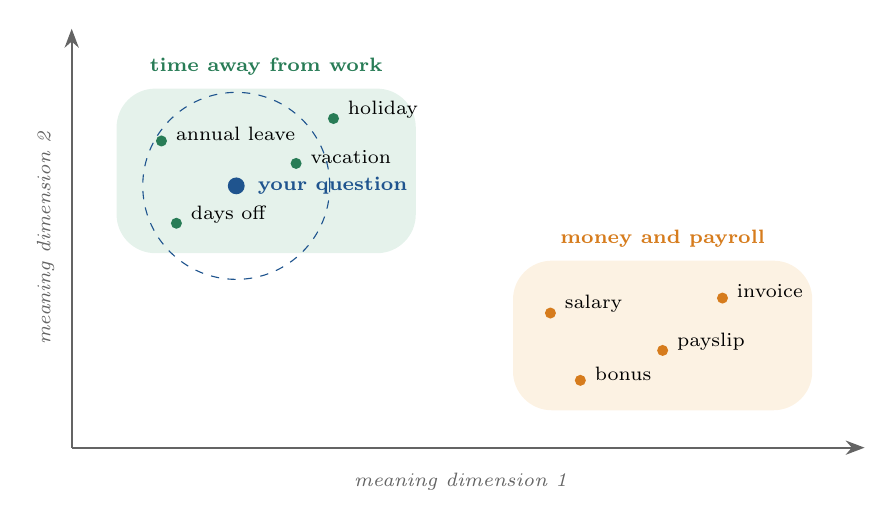
\begin{tikzpicture}[scale=0.95]
    \draw[ar] (0,0) -- (10.6,0);
    \draw[ar] (0,0) -- (0,5.6);
    \node[lbl, rotate=90] at (-0.35,2.8) {meaning dimension 2};
    \node[lbl] at (5.2,-0.45) {meaning dimension 1};

    \begin{scope}[on background layer]
      \fill[ragmint, rounded corners=14pt, opacity=0.85, visible on=<1->]
           (0.6,2.6) rectangle (4.6,4.8);
      \fill[ragsand, rounded corners=14pt, opacity=0.85, visible on=<2->]
           (5.9,0.5) rectangle (9.9,2.5);
    \end{scope}
    \node[font=\scriptsize\bfseries, text=raggreen, visible on=<1->]
         at (2.6,5.1) {time away from work};
    \node[font=\scriptsize\bfseries, text=ragorange, visible on=<2->]
         at (7.9,2.8) {money and payroll};

    \foreach \x/\y/\t in {1.2/4.1/{annual leave}, 3.0/3.8/{vacation},
                          1.4/3.0/{days off}, 3.5/4.4/{holiday}}{
      \fill[raggreen, visible on=<1->] (\x,\y) circle (2.1pt);
      \node[font=\scriptsize, above right=-1.2mm and 0.6mm, visible on=<1->]
           at (\x,\y) {\t};
    }
    \foreach \x/\y/\t in {6.4/1.8/{salary}, 7.9/1.3/{payslip},
                          6.8/0.9/{bonus}, 8.7/2.0/{invoice}}{
      \fill[ragorange, visible on=<2->] (\x,\y) circle (2.1pt);
      \node[font=\scriptsize, above right=-1.2mm and 0.6mm, visible on=<2->]
           at (\x,\y) {\t};
    }
    \draw[ragblue, dashed, visible on=<3->] (2.2,3.5) circle (1.25);
    \fill[ragblue, visible on=<3->] (2.2,3.5) circle (3.2pt);
    \node[font=\scriptsize\bfseries, text=ragblue, right=1.5mm, visible on=<3->]
         at (2.2,3.5) {your question};
  \end{tikzpicture}
  \end{center}
  \centering\small\color{raggray}
  \uncover<3->{Real maps have hundreds of dimensions instead of two --- but the
  idea is exactly this: \textbf{close together = similar meaning}.}
\end{frame}

%---- the one genuinely moving slide --------------------------
\begin{frame}{Retrieval in slow motion}
  \animate<2-14>
  \animatevalue<1-14>{\searchradius}{0cm}{2.0cm}
  \begin{center}
  \vspace{-4mm}
  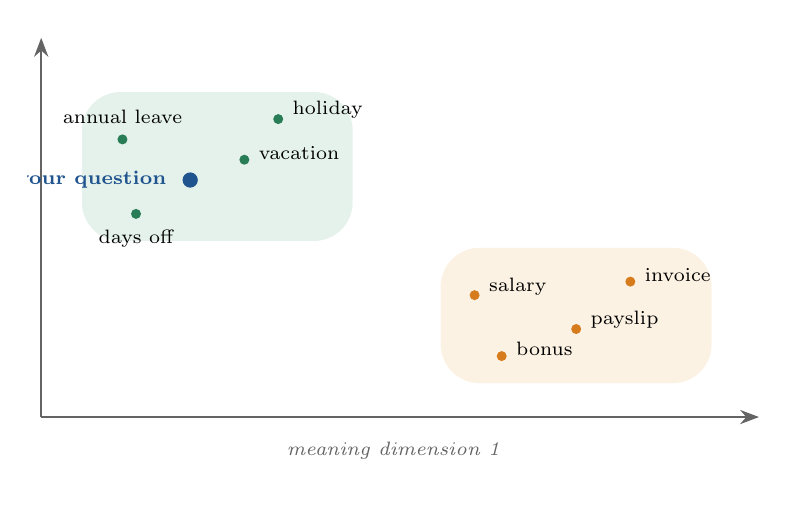
\begin{tikzpicture}[scale=0.86]
    % pin (and clip to) a fixed bounding box so the growing circle
    % can never change the size of the picture between slides
    \path[clip] (-0.2,-0.9) rectangle (10.9,5.75);

    \draw[ar] (0,0) -- (10.6,0);
    \draw[ar] (0,0) -- (0,5.6);
    \node[lbl] at (5.2,-0.5) {meaning dimension 1};

    \begin{scope}[on background layer]
      \fill[ragmint, rounded corners=14pt, opacity=0.85]
           (0.6,2.6) rectangle (4.6,4.8);
      \fill[ragsand, rounded corners=14pt, opacity=0.85]
           (5.9,0.5) rectangle (9.9,2.5);
    \end{scope}

    % the growing search radius
    \fill[ragblue, opacity=0.10] (2.2,3.5) circle (\the\searchradius);
    \draw[ragblue, dashed, thick] (2.2,3.5) circle (\the\searchradius);

    % green cluster: each point lights up as the circle reaches it
    \swallowpoint{3.0}{3.8}{vacation}{0.854cm}{above right=-1.2mm and 0.6mm}
    \swallowpoint{1.4}{3.0}{days off}{0.943cm}{below=0.8mm}
    \swallowpoint{1.2}{4.1}{annual leave}{1.166cm}{above=0.8mm}
    \swallowpoint{3.5}{4.4}{holiday}{1.581cm}{above right=-1.2mm and 0.6mm}
    % payroll cluster: never reached
    \foreach \x/\y/\t in {6.4/1.8/{salary}, 7.9/1.3/{payslip},
                          6.8/0.9/{bonus}, 8.7/2.0/{invoice}}{
      \fill[ragorange] (\x,\y) circle (2.1pt);
      \node[font=\scriptsize, above right=-1.2mm and 0.6mm] at (\x,\y) {\t};
    }

    \fill[ragblue] (2.2,3.5) circle (3.2pt);
    \node[font=\scriptsize\bfseries, text=ragblue, left=1.8mm]
         at (2.2,3.5) {your question};
  \end{tikzpicture}
  \end{center}
  \begin{minipage}[t][1.1cm]{\textwidth}
    \centering\small
    \only<1>{The dashed circle is how far we are willing to look.
             Watch it grow.}%
    \only<2-13>{\color{ragblue}Every point the circle swallows becomes a
             candidate passage.}%
    \only<14->{\color{raggreen}\textbf{The four nearest passages are the ones
             handed to the model} --- and nothing from payroll ever comes
             close.}
  \end{minipage}
\end{frame}

\begin{frame}{Measuring ``close''}
  For each stored passage we ask: how similar is its direction to the
  question's direction? That number is the \alert{similarity score}.
  \bigskip
  \begin{columns}[c,onlytextwidth]
    \begin{column}{0.401\textwidth}
      \centering
      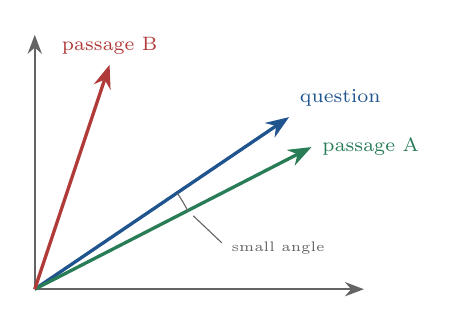
\begin{tikzpicture}[scale=0.95]
        \draw[ar] (0,0) -- (4.4,0);
        \draw[ar] (0,0) -- (0,3.4);
        \draw[-{Stealth}, very thick, ragblue] (0,0) -- (3.4,2.3)
              node[above right, font=\scriptsize, text=ragblue] {question};
        \draw[-{Stealth}, very thick, raggreen, visible on=<2->] (0,0) -- (3.7,1.9)
              node[right, font=\scriptsize, text=raggreen] {passage A};
        \draw[-{Stealth}, very thick, ragred, visible on=<3->] (0,0) -- (1.0,3.0)
              node[above, font=\scriptsize, text=ragred] {passage B};
        \draw[raggray, thin, visible on=<2->] (2.05,1.04) arc (27:34:2.3);
        \draw[raggray, thin, visible on=<2->] (2.5,0.62) -- (2.12,0.98);
        \node[font=\tiny, text=raggray, right, visible on=<2->]
             at (2.5,0.55) {small angle};
      \end{tikzpicture}
    \end{column}
    \begin{column}{0.554\textwidth}
      \begin{block}<4->{Reading the score}
        \begin{itemize}
          \item Small angle $\Rightarrow$ score near \textbf{1.0}
                $\Rightarrow$ very relevant
          \item Wide angle $\Rightarrow$ score near \textbf{0}
                $\Rightarrow$ unrelated
        \end{itemize}
      \end{block}
      \begin{exampleblock}<5->{So retrieval becomes arithmetic}
        Score every passage, sort the list, keep the top few.
        A computer can do this over millions of passages in
        milliseconds.
      \end{exampleblock}
    \end{column}
  \end{columns}
\end{frame}

\begin{frame}{Where the coordinates live: the vector database}
  \begin{columns}[T,onlytextwidth]
    \begin{column}{0.525\textwidth}
      A \alert{vector database} is a store built for one question:
      \begin{block}{}
        \centering ``Which stored items sit closest to \emph{this} point?''
      \end{block}
      \medskip
      \uncover<3->{Each row holds:}
      \begin{itemize}
        \item<3-> the numbers (the coordinates),
        \item<3-> the original text,
        \item<3-> bookkeeping: file name, page, date, who may read it.
      \end{itemize}
      \medskip
      \uncover<4->{That last part is what lets an answer say
      \emph{``Handbook, section 4.2''}.}
    \end{column}
    \begin{column}{0.43\textwidth}
      \centering
      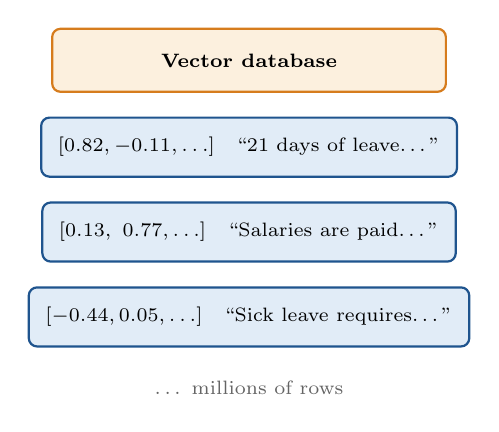
\begin{tikzpicture}[node distance=3mm]
        \node[obox, minimum width=5.0cm, font=\scriptsize, minimum height=0.8cm,
              visible on=<2->] (h) {\textbf{Vector database}};
        \node[box, below=of h, minimum width=5.0cm, font=\scriptsize,
              minimum height=0.75cm, visible on=<2->] (r1)
             {$[0.82,-0.11,\dots]$ \; ``21 days of leave\dots''};
        \node[box, below=of r1, minimum width=5.0cm, font=\scriptsize,
              minimum height=0.75cm, visible on=<2->] (r2)
             {$[0.13,\ 0.77,\dots]$ \; ``Salaries are paid\dots''};
        \node[box, below=of r2, minimum width=5.0cm, font=\scriptsize,
              minimum height=0.75cm, visible on=<2->] (r3)
             {$[-0.44,0.05,\dots]$ \; ``Sick leave requires\dots''};
        \node[font=\scriptsize, text=raggray, below=of r3, visible on=<2->]
             {\dots\ millions of rows};
      \end{tikzpicture}
    \end{column}
  \end{columns}
\end{frame}

%==============================================================
\section{Part 4 --- The full picture}

\begin{frame}{Stage 1: Preparation (done once, in advance)}
  \begin{center}
  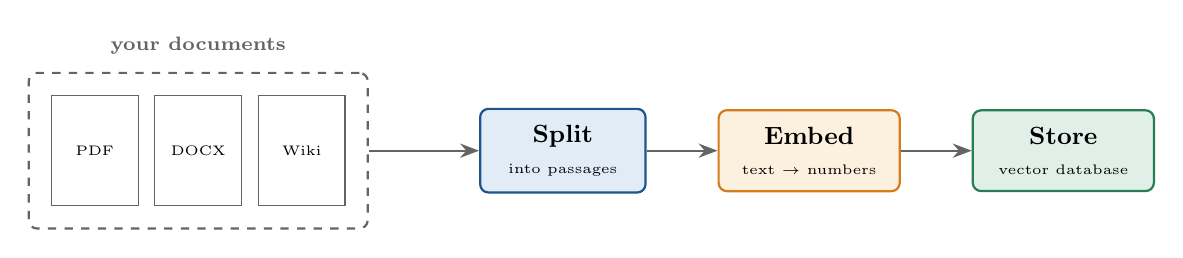
\begin{tikzpicture}[node distance=9mm]
    \node[doc] (d1) {PDF};
    \node[doc, right=2mm of d1] (d2) {DOCX};
    \node[doc, right=2mm of d2] (d3) {Wiki};
    \node[box, fit=(d1)(d2)(d3), inner sep=8pt, fill=none, draw=raggray,
          dashed] (docs) {};
    \node[above=1mm of docs, font=\scriptsize\bfseries, text=raggray]
         {your documents};

    \node[box, right=1.4cm of docs, minimum width=2.1cm, visible on=<2->]
         (chunk) {\textbf{Split}\\\tiny into passages};
    \node[obox, right=of chunk, minimum width=2.3cm, visible on=<3->] (emb)
         {\textbf{Embed}\\\tiny text $\to$ numbers};
    \node[gbox, right=of emb, minimum width=2.3cm, visible on=<4->] (db)
         {\textbf{Store}\\\tiny vector database};

    \draw[ar, visible on=<2->] (docs) -- (chunk);
    \draw[ar, visible on=<3->] (chunk) -- (emb);
    \draw[ar, visible on=<4->] (emb) -- (db);
  \end{tikzpicture}
  \end{center}
  \bigskip
  \begin{block}<5->{What happens here}
    \begin{enumerate}
      \item Collect the documents you want the AI to be able to consult.
      \item Cut them into passages of roughly a page or a paragraph.
      \item Convert every passage into its list of numbers.
      \item Save numbers $+$ text $+$ source information.
    \end{enumerate}
  \end{block}
  \centering\small\color{raggray}
  \uncover<5->{Repeated only when documents change --- nightly, hourly, or on
  upload.}
\end{frame}

\begin{frame}{Stage 2: Answering (every time someone asks)}
  \begin{center}
  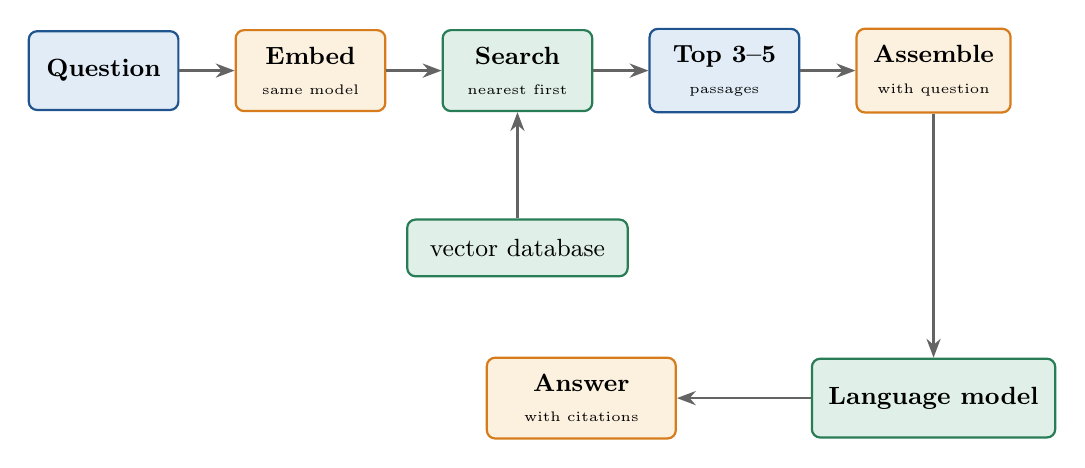
\begin{tikzpicture}[node distance=7mm]
    \node[box, minimum width=1.9cm] (q) {\textbf{Question}};
    \node[obox, right=of q, minimum width=1.9cm, visible on=<2->] (qe)
         {\textbf{Embed}\\\tiny same model};
    \node[gbox, right=of qe, minimum width=1.9cm, visible on=<3->] (search)
         {\textbf{Search}\\\tiny nearest first};
    \node[box, right=of search, minimum width=1.9cm, visible on=<4->] (top)
         {\textbf{Top 3--5}\\\tiny passages};
    \node[obox, right=of top, minimum width=1.9cm, visible on=<5->] (prompt)
         {\textbf{Assemble}\\\tiny with question};
    \node[box, below=1.35cm of search, minimum width=2.8cm, minimum height=0.72cm,
          fill=ragmint, draw=raggreen, visible on=<3->] (db)
         {\small vector database};
    \node[gbox, below=3.1cm of prompt, minimum width=2.4cm, visible on=<6->]
         (llm) {\textbf{Language model}};
    \node[box, left=1.7cm of llm, minimum width=2.4cm, fill=ragsand,
          draw=ragorange, visible on=<7->] (ans)
         {\textbf{Answer}\\\tiny with citations};

    \draw[ar, visible on=<2->] (q) -- (qe);
    \draw[ar, visible on=<3->] (qe) -- (search);
    \draw[ar, visible on=<3->] (db) -- (search);
    \draw[ar, visible on=<4->] (search) -- (top);
    \draw[ar, visible on=<5->] (top) -- (prompt);
    \draw[ar, visible on=<6->] (prompt) -- (llm);
    \draw[ar, visible on=<7->] (llm) -- (ans);
  \end{tikzpicture}
  \end{center}
  \centering\small\color{raggray}
  \uncover<7->{All of this happens in about a second, between the user pressing
  \emph{Enter} and the first word appearing.}
\end{frame}

\begin{frame}{Why we cut documents into passages}
  \begin{columns}[T,onlytextwidth]
    \begin{column}{0.478\textwidth}
      \begin{block}{Two hard limits}
        \begin{itemize}
          \item A model can only read so much text at once.
          \item Precision: you want \emph{the paragraph}, not
                \emph{the 400-page manual}.
        \end{itemize}
      \end{block}
      \begin{exampleblock}<3->{Rules of thumb}
        \begin{itemize}
          \item A passage $\approx$ a paragraph to a page
          \item Let neighbours overlap slightly, so a sentence
                split across the boundary is not lost
          \item Respect natural structure: headings, sections, slides
        \end{itemize}
      \end{exampleblock}
    \end{column}
    \begin{column}{0.478\textwidth}
      \centering
      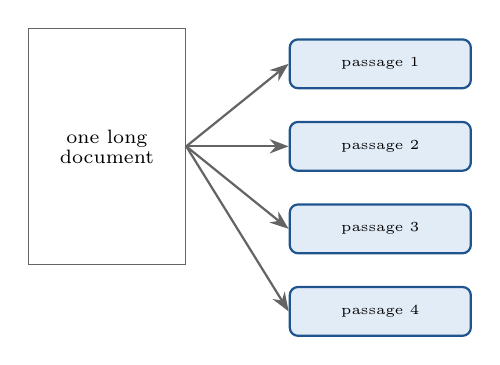
\begin{tikzpicture}[node distance=4mm]
        \node[doc, minimum width=2.0cm, minimum height=3.0cm] (big)
             {\scriptsize one long\\\scriptsize document};
        \node[box, right=1.3cm of big, minimum width=2.3cm,
              minimum height=0.62cm, visible on=<2->] (c2) {\tiny passage 2};
        \node[box, above=of c2, minimum width=2.3cm,
              minimum height=0.62cm, visible on=<2->] (c1) {\tiny passage 1};
        \node[box, below=of c2, minimum width=2.3cm,
              minimum height=0.62cm, visible on=<2->] (c3) {\tiny passage 3};
        \node[box, below=of c3, minimum width=2.3cm,
              minimum height=0.62cm, visible on=<2->] (c4) {\tiny passage 4};
        \draw[ar, visible on=<2->] (big.east) -- (c1.west);
        \draw[ar, visible on=<2->] (big.east) -- (c2.west);
        \draw[ar, visible on=<2->] (big.east) -- (c3.west);
        \draw[ar, visible on=<2->] (big.east) -- (c4.west);
      \end{tikzpicture}
      \medskip

      \small\color{raggray}
      \uncover<4->{Cut too small and you lose context; too big and you drown
      the model in irrelevant text.}
    \end{column}
  \end{columns}
\end{frame}

%==============================================================
\section{Part 5 --- A worked example}

\begin{frame}{The setting}
  \begin{block}{Scenario}
    A company puts its 300-page employee handbook behind an internal
    assistant. An employee types:
  \end{block}
  \begin{center}
    \begin{uncoverenv}<2->
    \begin{beamercolorbox}[sep=8pt,rounded=true,center,wd=0.75\textwidth]{block title example}
      \large ``How many days off do I get in my first year?''
    \end{beamercolorbox}
    \end{uncoverenv}
  \end{center}
  \medskip
  \begin{columns}[T,onlytextwidth]
    \begin{column}{0.478\textwidth}
      \begin{alertblock}<3->{A plain model would\dots}
        Answer from general knowledge --- ``typically around 20 days'' ---
        which may be wrong here, with no source.
      \end{alertblock}
    \end{column}
    \begin{column}{0.478\textwidth}
      \begin{exampleblock}<4->{A RAG system will\dots}
        Find the leave section of \emph{this} handbook and answer from it.
        Let us follow the four steps.
      \end{exampleblock}
    \end{column}
  \end{columns}
\end{frame}

\begin{frame}{Step 1 and 2 --- Embed the question, search the map}
  \begin{columns}[T,onlytextwidth]
    \begin{column}{0.42\textwidth}
      \textbf{Step 1.} The question becomes coordinates:
      \smallskip

      \begin{beamercolorbox}[sep=5pt,rounded=true]{block body}
        \small ``How many days off\dots'' \\
        $\Rightarrow [\,0.79,\ -0.08,\ 0.51,\ \dots\,]$
      \end{beamercolorbox}
      \medskip

      \uncover<2->{\textbf{Step 2.} We look for the nearest passages in the
      handbook --- \emph{not} for the words ``days off''.}
      \medskip

      \begin{exampleblock}<5->{Note}
        The winning passage never uses the phrase ``days off''.
        Keyword search would have missed it.
      \end{exampleblock}
    \end{column}
    \begin{column}{0.535\textwidth}
      \small\uncover<2->{\textbf{Top matches returned}}
      \smallskip

      \begin{uncoverenv}<3->
      \begin{beamercolorbox}[sep=5pt,rounded=true]{block body example}
        \scriptsize
        \textbf{0.91} --- \emph{Handbook \S4.2, Annual Leave}\\
        ``Employees accrue 21 days of annual leave per year, pro-rated in the
        first year of service.''
      \end{beamercolorbox}
      \end{uncoverenv}
      \smallskip
      \begin{uncoverenv}<4->
      \begin{beamercolorbox}[sep=5pt,rounded=true]{block body}
        \scriptsize
        \textbf{0.84} --- \emph{Handbook \S4.5, Public Holidays}\\
        ``In addition, 11 public holidays are observed.''
      \end{beamercolorbox}
      \end{uncoverenv}
      \smallskip
      \begin{uncoverenv}<4->
      \begin{beamercolorbox}[sep=5pt,rounded=true]{block body}
        \scriptsize
        \textbf{0.61} --- \emph{Handbook \S4.7, Sick Leave}\\
        ``Sick leave is granted separately and requires\dots''
      \end{beamercolorbox}
      \end{uncoverenv}
      \smallskip
      \begin{uncoverenv}<4->
      \begin{beamercolorbox}[sep=5pt,rounded=true]{block body}
        \scriptsize
        \textbf{0.22} --- \emph{Handbook \S9.1, Parking}\ \ (ignored)
      \end{beamercolorbox}
      \end{uncoverenv}
    \end{column}
  \end{columns}
\end{frame}

\begin{frame}{Step 3 --- Assemble what the model actually receives}
  \begin{beamercolorbox}[sep=9pt,rounded=true]{block body}
    \small
    \textbf{\color{ragblue}Instructions.}
    You are an HR assistant. Answer the question using only the context
    below. Cite the section you used. If the context does not contain the
    answer, say that you do not know.

    \medskip
    \onslide<2->
    \textbf{\color{ragorange}Context.}\\
    {}[\S4.2 Annual Leave] Employees accrue 21 days of annual leave per year,
    pro-rated in the first year of service.\\
    {}[\S4.5 Public Holidays] In addition, 11 public holidays are observed.\\
    {}[\S4.7 Sick Leave] Sick leave is granted separately and requires\dots

    \medskip
    \onslide<3->
    \textbf{\color{raggreen}Question.}
    How many days off do I get in my first year?
  \end{beamercolorbox}
  \medskip
  \centering\small\color{raggray}
  \uncover<4->{This assembled text is the whole ``augmentation''. Nothing about
  the model itself was modified.}
\end{frame}

\begin{frame}{Step 4 --- The answer}
  \begin{beamercolorbox}[sep=9pt,rounded=true]{block body example}
    You accrue \textbf{21 days of annual leave} per full year. In your first
    year this is \textbf{pro-rated}, so the amount depends on your start
    date. Separately, the company observes \textbf{11 public holidays}.
    \medskip

    \onslide<2->
    \small\emph{Sources: Handbook \S4.2 (Annual Leave), \S4.5 (Public
    Holidays).}
  \end{beamercolorbox}
  \bigskip
  \begin{columns}[T,onlytextwidth]
    \begin{column}{0.478\textwidth}
      \begin{block}<3->{What made this good}
        \begin{itemize}
          \item Numbers came from the handbook, not from memory
          \item Sources let the reader verify
          \item Update the handbook $\Rightarrow$ the answer updates
        \end{itemize}
      \end{block}
    \end{column}
    \begin{column}{0.478\textwidth}
      \begin{exampleblock}<4->{And if the handbook were silent?}
        The instruction told the model to say it does not know --- far more
        useful than a confident guess.
      \end{exampleblock}
    \end{column}
  \end{columns}
\end{frame}

%==============================================================
\section{Part 6 --- Trade-offs, pitfalls, and where it is used}

\begin{frame}{What RAG buys you}
  \begin{columns}[T,onlytextwidth]
    \begin{column}{0.478\textwidth}
      \begin{exampleblock}{Strengths}
        \begin{itemize}[<+->]
          \item \textbf{Current:} answers reflect today's documents
          \item \textbf{Private:} your own data, without retraining anything
          \item \textbf{Verifiable:} citations by construction
          \item \textbf{Cheap to maintain:} edit a file, not a model
          \item \textbf{Governable:} you decide what is in the collection ---
                and who may see what
        \end{itemize}
      \end{exampleblock}
    \end{column}
    \begin{column}{0.478\textwidth}
      \begin{block}<6->{The alternative: retraining}
        Baking new knowledge into the model itself is slow, expensive,
        needs specialists, and has to be redone whenever facts change ---
        and it still gives you no citations.
        \medskip

        RAG changes the \emph{input}, not the model. That is why it became
        the default way to put an LLM to work on real documents.
      \end{block}
    \end{column}
  \end{columns}
\end{frame}

\begin{frame}{What can still go wrong}
  \begin{columns}[T,onlytextwidth]
    \begin{column}{0.478\textwidth}
      \begin{alertblock}{Retrieval problems}
        \begin{itemize}
          \item \textbf{Missed it:} the right passage was never returned ---
                the answer cannot be right
          \item \textbf{Noise:} five loosely related passages crowd out the
                one that mattered
          \item \textbf{Stale collection:} nobody re-indexed after the update
          \item \textbf{Bad input:} scanned PDFs and tables that convert to
                gibberish
        \end{itemize}
      \end{alertblock}
    \end{column}
    \begin{column}{0.478\textwidth}
      \begin{alertblock}<2->{Generation problems}
        \begin{itemize}
          \item The model drifts beyond the passages it was given
          \item Two passages contradict each other and it picks one silently
          \item Confident tone hides a weak source
        \end{itemize}
      \end{alertblock}
      \begin{block}<3->{The rule}
        \centering
        Garbage in, garbage cited. \\
        RAG grounds the model --- it does not make it infallible.
      \end{block}
    \end{column}
  \end{columns}
\end{frame}

\begin{frame}{Making it work well in practice}
  \begin{columns}[T,onlytextwidth]
    \begin{column}{0.478\textwidth}
      \begin{block}{Get the boring things right}
        \begin{itemize}
          \item Clean, well-structured source documents
          \item Sensible passage sizes; keep headings with their text
          \item Keep the index fresh, automatically
          \item Enforce permissions \emph{during} retrieval, not after
        \end{itemize}
      \end{block}
    \end{column}
    \begin{column}{0.478\textwidth}
      \begin{block}<2->{Common improvements}
        \begin{itemize}[<+(1)->]
          \item \textbf{Hybrid search:} meaning-based \emph{plus} keyword ---
                good for names, codes, part numbers
          \item \textbf{Re-ranking:} fetch 50 candidates, then have a second,
                pickier model choose the best 5
          \item \textbf{Show sources in the interface} so users can check
          \item \textbf{Measure:} keep a set of real questions with known
                answers and test after every change
        \end{itemize}
      \end{block}
    \end{column}
  \end{columns}
\end{frame}

\begin{frame}{Where you have probably already met it}
  \begin{columns}[T,onlytextwidth]
    \begin{column}{0.478\textwidth}
      \begin{block}{Everyday}
        \begin{itemize}
          \item Chatbots that answer with a link to the help article
          \item ``Search your files'' assistants in office suites
          \item AI answers that cite web pages
        \end{itemize}
      \end{block}
    \end{column}
    \begin{column}{0.478\textwidth}
      \begin{block}<2->{Professional}
        \begin{itemize}
          \item \textbf{Legal:} question a contract archive
          \item \textbf{Medical:} guidelines and patient history
          \item \textbf{Engineering:} maintenance manuals on the shop floor
          \item \textbf{Finance:} filings, policies, audit trails
          \item \textbf{Support:} tickets and past resolutions
        \end{itemize}
      \end{block}
    \end{column}
  \end{columns}
  \medskip
  \begin{exampleblock}<3->{The tell}
    If an AI answer comes with a citation you can click, something like RAG is
    almost certainly running underneath.
  \end{exampleblock}
\end{frame}

%==============================================================
\section{Part 7 --- A real build, start to finish}

\begin{frame}{This is not hypothetical}
  \begin{block}{One evening, one ordinary laptop}
    Everything in this talk so far has been diagrams. This part is a real
    story: pointing a home PC at a folder of documents and building a working
    RAG from nothing, in one sitting.
  \end{block}
  \medskip
  \begin{columns}[T,onlytextwidth]
    \begin{column}{0.478\textwidth}
      \begin{exampleblock}<2->{The hardware}
        \begin{itemize}
          \item An ordinary gaming PC
          \item One graphics card with 8\,GB of memory
          \item No data centre, no cloud bill
        \end{itemize}
      \end{exampleblock}
    \end{column}
    \begin{column}{0.478\textwidth}
      \begin{exampleblock}<3->{The tools (all free)}
        \begin{itemize}
          \item A small language model, run locally
          \item A small embedding model, run locally
          \item A vector database on the same machine
        \end{itemize}
      \end{exampleblock}
    \end{column}
  \end{columns}
  \medskip
  \uncover<4->{\centering\small\color{raggray}
  The point is not the specific tools --- it's that everything you've just
  learned fits on a single consumer PC.}
\end{frame}

\begin{frame}{The build: the same five steps, for real}
  \centering
  \begin{beamercolorbox}[sep=8pt,rounded=true,wd=0.92\textwidth]{block body}
    \ttfamily\footnotesize
    install a local model runner \\
    download a small language model \ +\ a small embedding model \\
    pip install (two small packages) \\
    \color{ragorange}> program.py ingest C:\textbackslash my\_documents \\
    \color{raggreen}> program.py chat
  \end{beamercolorbox}
  \bigskip
  \begin{block}<2->{Nothing new, conceptually}
    \texttt{ingest} is Stage 1 from earlier: split, embed, store.
    \texttt{chat} is Stage 2: embed the question, search, assemble, generate.
    Same five moving parts, just typed instead of drawn.
  \end{block}
  \medskip
  \centering\small\color{raggray}
  \uncover<3->{Total setup time: about fifteen minutes, mostly spent
  downloading.}
\end{frame}

\begin{frame}{The first question --- and the first failure}
  \begin{block}{The question that was supposed to be easy}
    \centering\large ``How do I keep a model loaded in memory?''
  \end{block}
  \medskip
  \uncover<2->{The answer sat almost word-for-word in one FAQ file. This
  should have been the safest question of the whole test.}
  \bigskip
  \begin{alertblock}<3->{What actually happened}
    The system answered anyway --- confidently, fluently, and from the
    \emph{wrong} file. Every retrieved passage came from a different
    document. The one file that actually had the answer never showed up at
    all.
  \end{alertblock}
  \medskip
  \uncover<4->{\centering\textbf{\color{ragblue}Welcome to a real RAG
  incident.}}
\end{frame}

\begin{frame}{Anatomy of a RAG incident}
  A wrong answer can only be born in three places --- and the fix is
  completely different for each one.
  \bigskip
  \begin{center}
  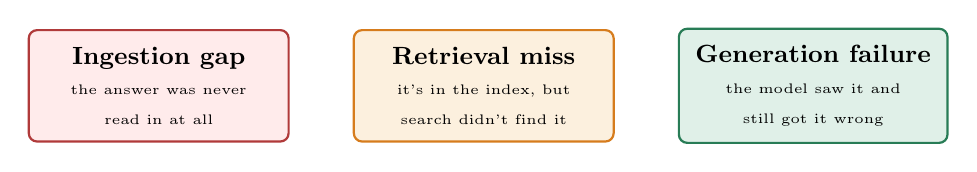
\begin{tikzpicture}[node distance=8mm]
    \node[rbox, minimum width=3.3cm, visible on=<2->] (ing)
         {\textbf{Ingestion gap}\\\tiny the answer was never\\\tiny read in
         at all};
    \node[obox, right=of ing, minimum width=3.3cm, visible on=<3->] (ret)
         {\textbf{Retrieval miss}\\\tiny it's in the index, but\\\tiny
         search didn't find it};
    \node[gbox, right=of ret, minimum width=3.3cm, visible on=<4->] (gen)
         {\textbf{Generation failure}\\\tiny the model saw it and\\\tiny
         still got it wrong};
  \end{tikzpicture}
  \end{center}
  \bigskip
  \uncover<5->{\begin{exampleblock}{The check that separates them}
    Before guessing: ask the store directly which files it actually holds.
    That one query tells you instantly whether you have an ingestion problem
    or something further downstream.
  \end{exampleblock}}
\end{frame}

\begin{frame}{The bug: one silent letter}
  \begin{center}
  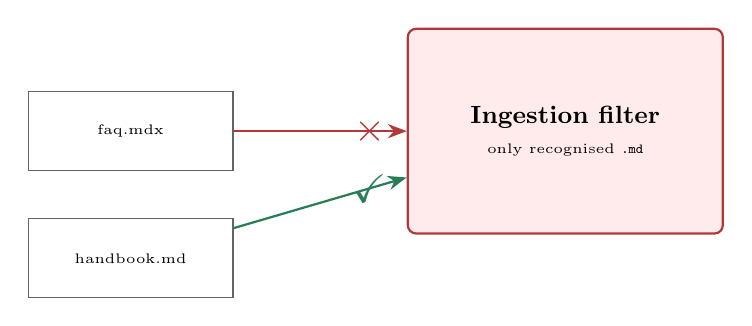
\begin{tikzpicture}[node distance=6mm]
    \node[doc, minimum width=2.6cm, minimum height=1cm, visible on=<1->]
         (file) {faq.mdx};
    \node[doc, below=of file, minimum width=2.6cm, minimum height=1cm,
          visible on=<3->] (other) {handbook.md};
    \node[rbox, right=2.2cm of file, minimum width=4.0cm, minimum height=2.6cm,
          visible on=<2->] (filter)
         {\textbf{Ingestion filter}\\\tiny only recognised \texttt{.md}};
    \draw[ar, ragred, visible on=<2->] (file) -- (filter);
    \node[font=\Large, text=ragred, visible on=<2->]
         at ($(file)!0.55!(filter)$) {$\times$};
    \draw[ar, raggreen, visible on=<3->] (other) -- (filter);
    \node[font=\Large, text=raggreen, visible on=<3->]
         at ($(other)!0.55!(filter)$) {$\checkmark$};
  \end{tikzpicture}
  \end{center}
  \bigskip
  \begin{alertblock}<4->{The actual cause}
    The FAQ file was named with an extra letter --- \texttt{.mdx}, not
    \texttt{.md}. The filter only watched for one exact spelling. The file
    was silently skipped, and the pipeline reported success anyway.
  \end{alertblock}
  \medskip
  \uncover<5->{\centering\small\color{raggray}
  Not embeddings, not the model, not the database. A file extension.}
\end{frame}

\begin{frame}{The lesson: garbage in is invisible}
  \begin{block}{Why this bug is the scary kind}
    Nothing crashed. No error appeared. The system ran end to end and gave a
    fluent, wrong answer --- which is worse than a crash, because a crash at
    least tells you to look.
  \end{block}
  \medskip
  \begin{columns}[T,onlytextwidth]
    \begin{column}{0.478\textwidth}
      \begin{exampleblock}<2->{The fix}
        Widen the filter to catch the file, then re-run ingestion. One
        line. The rest of the pipeline was already correct.
      \end{exampleblock}
    \end{column}
    \begin{column}{0.478\textwidth}
      \begin{block}<3->{The habit that catches it next time}
        Have ingestion report its own coverage: \emph{found 214 files,
        indexed 198, skipped 16}. A silent gap should scream, not hide.
      \end{block}
    \end{column}
  \end{columns}
  \medskip
  \uncover<4->{\centering\textbf{\color{ragblue}This is ``garbage in,
  garbage cited'' from earlier --- happening for real.}}
\end{frame}

\begin{frame}{Plot twist: one word, two meanings}
  \begin{block}{The setup}
    The same system was now loaded with two unrelated document sets: a
    data-tool's documentation, and the AI model-runner's own documentation.
    Both use one word constantly: \textbf{model}.
  \end{block}
  \medskip
  \begin{center}
  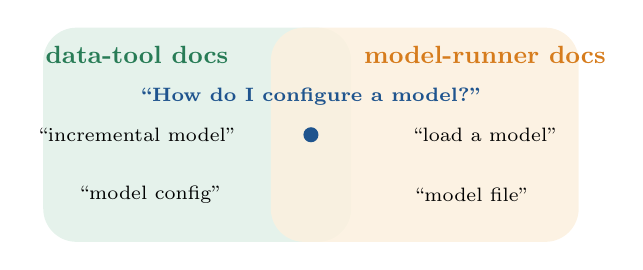
\begin{tikzpicture}[scale=0.85]
    \fill[ragmint, rounded corners=12pt, opacity=0.85, visible on=<2->]
         (0,0) rectangle (4.6,3.2);
    \fill[ragsand, rounded corners=12pt, opacity=0.85, visible on=<3->]
         (3.4,0) rectangle (8.0,3.2);
    \node[font=\small\bfseries, text=raggreen, visible on=<2->] at (1.4,2.8)
         {data-tool docs};
    \node[font=\small\bfseries, text=ragorange, visible on=<3->] at (6.6,2.8)
         {model-runner docs};
    \node[font=\scriptsize, visible on=<2->] at (1.4,1.6) {``incremental model''};
    \node[font=\scriptsize, visible on=<2->] at (1.6,0.7) {``model config''};
    \node[font=\scriptsize, visible on=<3->] at (6.6,1.6) {``load a model''};
    \node[font=\scriptsize, visible on=<3->] at (6.4,0.7) {``model file''};
    \fill[ragblue, visible on=<4->] (4.0,1.6) circle (3.2pt);
    \node[font=\scriptsize\bfseries, text=ragblue, above, visible on=<4->]
         at (4.0,1.9) {``How do I configure a model?''};
  \end{tikzpicture}
  \end{center}
  \uncover<5->{\centering\small
  The question lands squarely in \textbf{both} clusters at once --- meaning
  alone cannot tell them apart.}
\end{frame}

\begin{frame}{The result: a confused search}
  \begin{alertblock}{What came back}
    A mixed bag: some passages about the data tool, some about the
    model-runner, none of them decisively winning. Not because retrieval was
    broken --- because the question was genuinely ambiguous, and embeddings
    can only match meaning, not intent.
  \end{alertblock}
  \smallskip
  \uncover<2->{\begin{block}{This has a name}
    \centering \textbf{Corpus collision} --- two unrelated document sets
    that happen to share vocabulary. It's the ``Noise'' failure from
    earlier, caught in the act.
  \end{block}}
  \smallskip
  \uncover<3->{\begin{exampleblock}{The fix}
    Remember the vector database's bookkeeping --- file name, source, date?
    Tag every chunk with \emph{which} document set it came from, then
    restrict a search to one tag before it even runs. One filter, and the
    ambiguity disappears --- like searching only one shelf of a library
    instead of the whole building.
  \end{exampleblock}}
\end{frame}

\begin{frame}{The road beyond this build}
  Everything above was the minimum viable version. Each pitfall from
  earlier has a real, learnable fix once you go looking for it:
  \begin{itemize}[<+->]
    \item Chunking that respects headings and structure, not just
          character counts
    \item Choosing and tuning the embedding model for your language and
          domain
    \item A proper database instead of a toy store, once the collection
          grows
    \item Combining meaning-search with old-fashioned keyword search, for
          the exact terms embeddings blur
    \item Teaching the model to cite sources and answer partially instead
          of refusing outright
    \item A small labelled test set, so ``I improved it'' becomes a
          number instead of a feeling
  \end{itemize}
  \medskip
  \uncover<7->{\centering\small\color{raggray}
  None of this changes the core idea. It's the same open-book exam, tuned.}
\end{frame}

\begin{frame}{You already have everything you need}
  \begin{block}{The whole recipe, again}
    A folder of documents you know well. A small local model. A few free
    tools. An afternoon.
  \end{block}
  \medskip
  \begin{exampleblock}<2->{Try it yourself}
    \begin{itemize}
      \item Pick 3--5 documents you actually know
      \item Ingest them, then ask it something easy --- confirm the basics
            work
      \item Then try to break it: an ambiguous question, a question the
            docs don't cover, a question that spans two files
      \item Every failure you find maps to something in this talk
    \end{itemize}
  \end{exampleblock}
  \medskip
  \uncover<3->{\centering\textbf{\color{ragblue}Your failures will teach you
  faster than any slide can.}}
\end{frame}

%==============================================================
\section{Wrap-up}

\begin{frame}{The vocabulary you now own}
  \begin{columns}[T,onlytextwidth]
    \begin{column}{0.478\textwidth}
      \begin{block}{}
        \small
        \textbf{LLM} --- software that continues text plausibly; the writer.
        \medskip

        \onslide<2->
        \textbf{Hallucination} --- a fluent answer that is simply not true.
        \medskip

        \onslide<3->
        \textbf{Embedding} --- meaning expressed as a list of numbers; an
        address on a map of meaning.
      \end{block}
    \end{column}
    \begin{column}{0.478\textwidth}
      \begin{block}<4->{}
        \small
        \textbf{Chunk / passage} --- a small piece of a document, the unit we
        search over.
        \medskip

        \onslide<5->
        \textbf{Vector database} --- a store that finds the nearest
        coordinates fast.
        \medskip

        \onslide<6->
        \textbf{RAG} --- search first, then answer from what was found.
      \end{block}
    \end{column}
  \end{columns}
  \medskip
  \begin{exampleblock}<7->{}
    \centering
    Closed-book exam $\rightarrow$ open-book exam. That is the whole idea.
  \end{exampleblock}
\end{frame}

\begin{frame}[plain]
  \transfade
  \vfill
  \centering
  {\Huge\bfseries\color{ragblue} Thank you}
  \vskip 8mm
  {\large Questions?}
  \vskip 12mm
  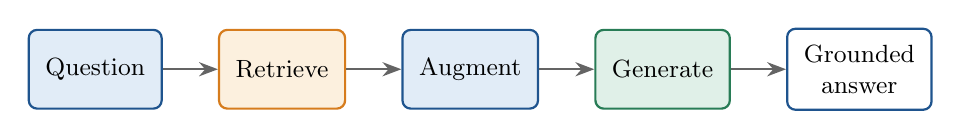
\begin{tikzpicture}[node distance=7mm]
    \node[box, visible on=<2->] (q) {Question};
    \node[obox, right=of q, visible on=<3->] (r) {Retrieve};
    \node[box, right=of r, visible on=<4->] (a) {Augment};
    \node[gbox, right=of a, visible on=<5->] (g) {Generate};
    \node[box, right=of g, fill=white, visible on=<6->] (ans)
         {Grounded\\answer};
    \draw[ar, visible on=<3->] (q) -- (r);
    \draw[ar, visible on=<4->] (r) -- (a);
    \draw[ar, visible on=<5->] (a) -- (g);
    \draw[ar, visible on=<6->] (g) -- (ans);
  \end{tikzpicture}
  \vfill
\end{frame}

\end{document}
